%%
%% results.tex
\forcecommand{\thesec}{Results}
\section{\thesec}
\label{sec:results}
%%

%%
%% progress
\begin{frame}{Work Completed}{}
  \vspace*{-2\baselineskip}
  \begin{itemize}
    \item{
      gain familiarity with and understanding of the SPH methodology
    }
    \item{
      gain proficiency with SPH software DualSPHysics
      \begin{itemize}
          \item{
            generation of complex computational domains and boundary geometries
          }
          \item{
            familiarity with tuning SPH simulation parameters and running of simulations
          }
          \item{
            analysis of simulation data
          }
      \end{itemize}
    }
    \item{
      implementation of surface tension model into DualSPHysics
      \begin{itemize}
        \item{
          gain familiarity with DualSPHysics source code and inner workings
        }
      \end{itemize}
    }
    \item{
      run simulations to test results produced by modified code against theory and experiment
    }
  \end{itemize}
\end{frame}

\begin{frame}{\thesec}{Summary of Results}
  \vspace*{-2\baselineskip}
  \begin{itemize}
    \item{
      excellent quantitative and qualitative agreement with theory in simulations of oscillating droplets
    }
    \vspace*{\baselineskip}
    \item{
      qualitative agreement with observed behavior in simulations of colliding droplets (quantitative data not available)
    }
    \vspace*{\baselineskip}
    \item{
      \alert{poor agreement with experimental results in simulations of fluid-solid impacts}
    }
  \end{itemize}
\end{frame}

%%
%% elliptical droplet oscillations
\begin{frame}{\thesec}{Elliptical Droplet Oscillations}
  \vspace*{-2.1\baselineskip}
  \begin{columns}
    \begin{column}{0.5\textwidth}
      \begin{figure}
        \centering
        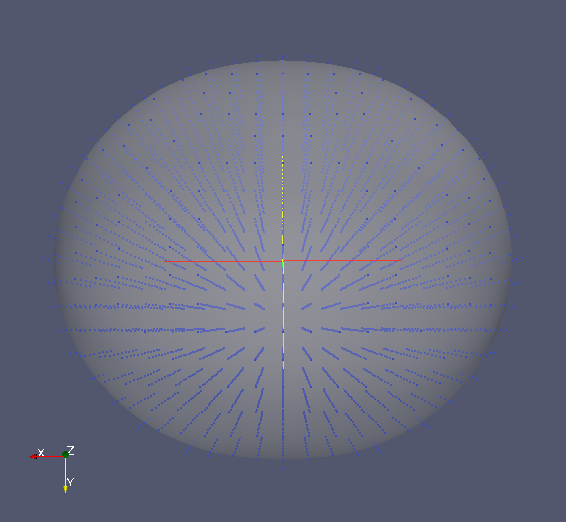
\includegraphics[width=\textwidth]{img/oscdrop0.png}
      \end{figure}
    \end{column}
    \begin{column}{0.5\textwidth}
      \begin{figure}
        \centering
        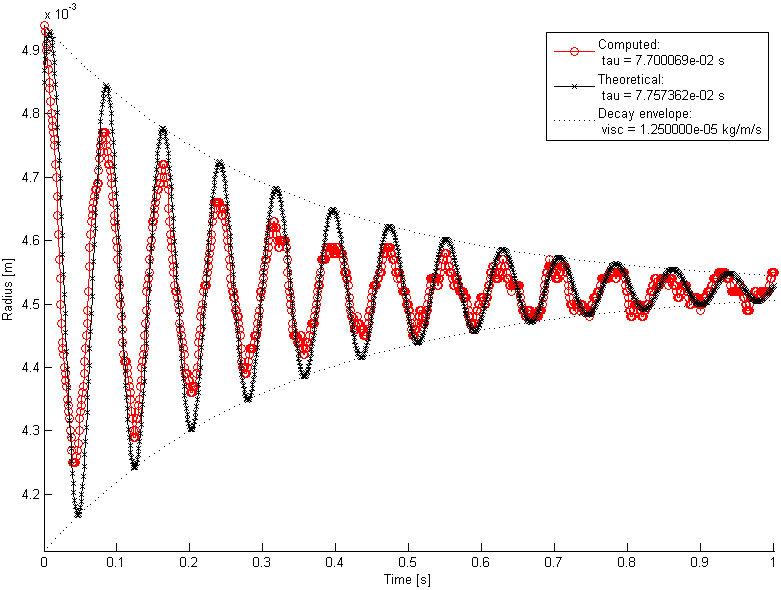
\includegraphics[width=\textwidth]{img/oscdrop_rad.png}
      \end{figure}
    \end{column}
  \end{columns}
\end{frame}

\begin{frame}{\thesec}{Fluid-Solid Impacts}
  \vspace*{-2.1\baselineskip}
  \begin{columns}
    \begin{column}{0.5\textwidth}
      \begin{figure}
        \centering
        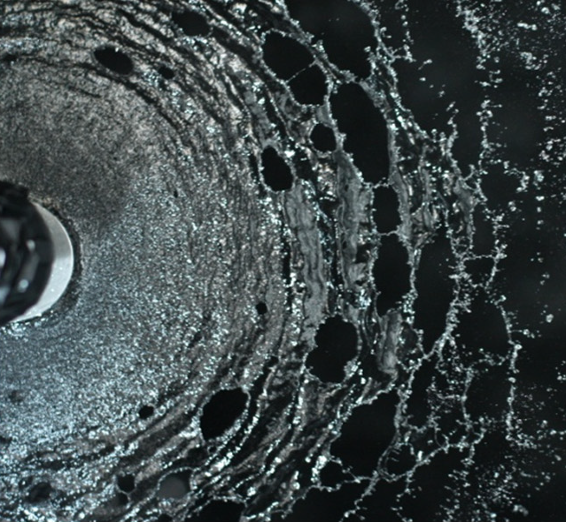
\includegraphics[width=\textwidth]{img/flappingSheetBreakup2_sm.png}
      \end{figure}
    \end{column}
    \begin{column}{0.5\textwidth}
      \begin{figure}
        \centering
        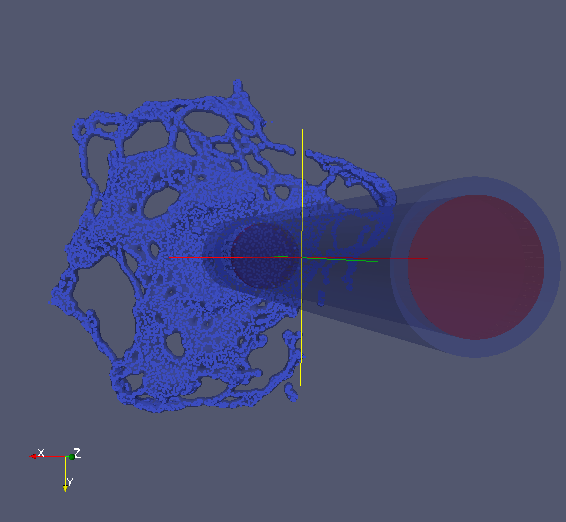
\includegraphics[width=\textwidth]{img/ren_marshall_far.png}
      \end{figure}
    \end{column}
  \end{columns}
\end{frame}
%% M. Sullivan. June, 2016